\documentclass[a4paper,12pt]{report}
\usepackage{amsmath}
\usepackage{subcaption}
\usepackage[utf8]{inputenc}
\usepackage[T1]{fontenc}
\usepackage{xcolor,graphicx}
\usepackage[top=0.6in,bottom=0.6in,right=1in,left=1in]{geometry}
\usepackage{color}
\usepackage{listings}

\begin{document}
\begin{titlepage}
    % \pagecolor{blue!10}
    \begin{center}
        \begin{minipage}{2.5cm}
        \begin{center}
            
\includegraphics[width=2.3cm,height=2.5cm]{slogan.jpg}
        \end{center}
    \end{minipage}\hfill
    \begin{minipage}{10cm}
        \begin{center}
      {\bfseries\large Cairo University - Faculty of Engineering}\\[0.1cm]
      {\bfseries\large Computer Engineering Department}\\[0.1cm]
      \end{center}
    
    \end{minipage}\hfill
    \begin{minipage}{2.5cm}
        \begin{center}
            
\includegraphics[width=2.5cm,height=2cm]{logo_cufe.png}
        \end{center}
    
    \end{minipage}
    
    \vspace{5cm}
    
    {\Huge \bfseries \uppercase{M-ary Amplitiude Shift Modulation} \\[0.5cm] }
    {\LARGE \bfseries Subject: Digital Communication}
    \textsc{\Large }\\[1cm]
    
    \vspace{5cm}
    
    % Author and supervisor
    \begin{minipage}{15cm}
      \begin{flushleft} \huge
        \emph{Submitted to:}\\
        Dr.~Hala \textsc{Abdel Kader}\\
        Dr.~Mai \textsc{Badawi}\\
      \end{flushleft}
    \end{minipage}
    
    \vspace{2cm}
    
    
    {\huge \textit{Presented by: }}\\[0.5cm]
    
    \color{black}
    \centering
    \begin{tabular}{lll}
    \large Evram \textsc{Youssef} : & \large Sec: 1 & \large BN: 9 \\[0.1cm]
    
    \end{tabular}

    \vspace{-0.5cm}

    \begin{figure}[h]
        %I put \linewidth into the brackets, which means the picture will be scaled to fit the width of the document.
        \centerline{
\includegraphics[width=5cm]{Figures/evram.JPG}}
    \end{figure}

    % Bottom of the page
    {\LARGE {Year}\\ 2019/2020}
    \end{center}
    \end{titlepage}


    \pagenumbering{gobble}
    \newpage
    \pagenumbering{arabic}

    \pagenumbering{gobble}
    \tableofcontents
    \listoffigures
    \newpage
    \pagenumbering{arabic}


    \section{Part 1: Digital Communication}
        
    \subsection{Problem 1}
        Figure 1 below showing the comparison between simulated BER and theoritical (analytical) BER
        VS the Eb/N0 in db.

        Please notice, you'll have to input the no. 
            of bits you wish to be transmitted, and it has to be divisible by 3.

    \subsection{Problem 2}
        The constellation of the 8-ary with decision region pf each symbol.

        Boundaries are at:
        \begin{equation*}
            -6 \sqrt{E}, -4 \sqrt{E}, -2 \sqrt{E}, 0, 2 \sqrt{E}, 4 \sqrt{E}, 6 \sqrt{E}
        \end{equation*}
        \vspace{-1cm}
        \begin{figure}[h!]
            %I put \linewidth into the brackets, which means the picture will be scaled to fit the width of the document.
            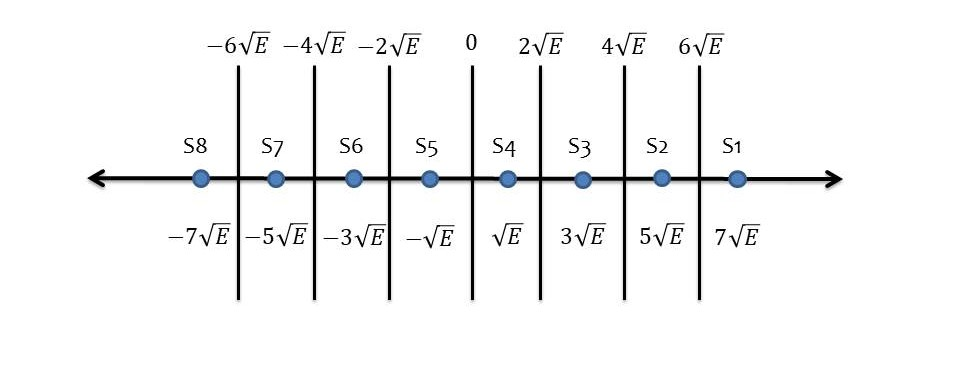
\includegraphics[width=\linewidth]{Figures/Figure_2.jpg}
            \caption{Symbols Boundary}
            \label{fig:Symbols}
        \end{figure}

    \vspace{1cm}

    \subsection{Problem 3}
        The derivation of theoritical bit error rate using 8-ary.
        \begin{equation}
            Pe = \frac{1}{8} \displaystyle\sum_{i=0}^{7} P(e|Si) 
        \end{equation}
        \begin{equation}
            Pe(e|S0) = Pe(e|S7)
        \end{equation}
        \begin{equation}
            Pe(e|S1) = Pe(e|S2) = Pe(e|S3) = Pe(e|S4) = Pe(e|S5) = Pe(e|S6)
        \end{equation}
        Using Union bound S0 and S7 has only one neighbour and S1, S2,...S6 has two neighbours.
        \begin{equation}
            Pe(e|S0) = \frac{1}{2} erfc(\frac{\sqrt{E}}{\sqrt{N}})
        \end{equation}
        \begin{equation}
            Pe(e|S1) = \frac{1}{2} erfc(\frac{\sqrt{E}}{\sqrt{N}})
                + \frac{1}{2} erfc(\frac{\sqrt{E}}{\sqrt{N}})
        \end{equation}
        \begin{equation}
            Pe(e|S1) = erfc(\frac{\sqrt{E}}{\sqrt{N}})
        \end{equation}
        \begin{equation}
            Pe = \frac{1}{8} (2 * \frac{1}{2} erfc(\frac{\sqrt{E}}{\sqrt{N}}) 
                + 6 * erfc(\frac{\sqrt{E}}{\sqrt{N}}))
        \end{equation}
        \begin{equation}
            Pe = \frac{7}{8} erfc(\frac{\sqrt{E}}{\sqrt{N}}) 
        \end{equation}

        So, BER (per bit) will be:
        \begin{equation}
            BER = \frac{Pe}{3}
        \end{equation}
        \begin{equation}
            BER = \frac{7}{24} (erfc(\frac{\sqrt{E}}{\sqrt{N}}))
        \end{equation}

    
    \subsection{Probelm 4}
        Figure 1 below showing the comparison between simulated BER and theoritical (analytical) BER
        VS the Eb/N0 in db.
        \begin{figure}[h!]
            %I put \linewidth into the brackets, which means the picture will be scaled to fit the width of the document.
            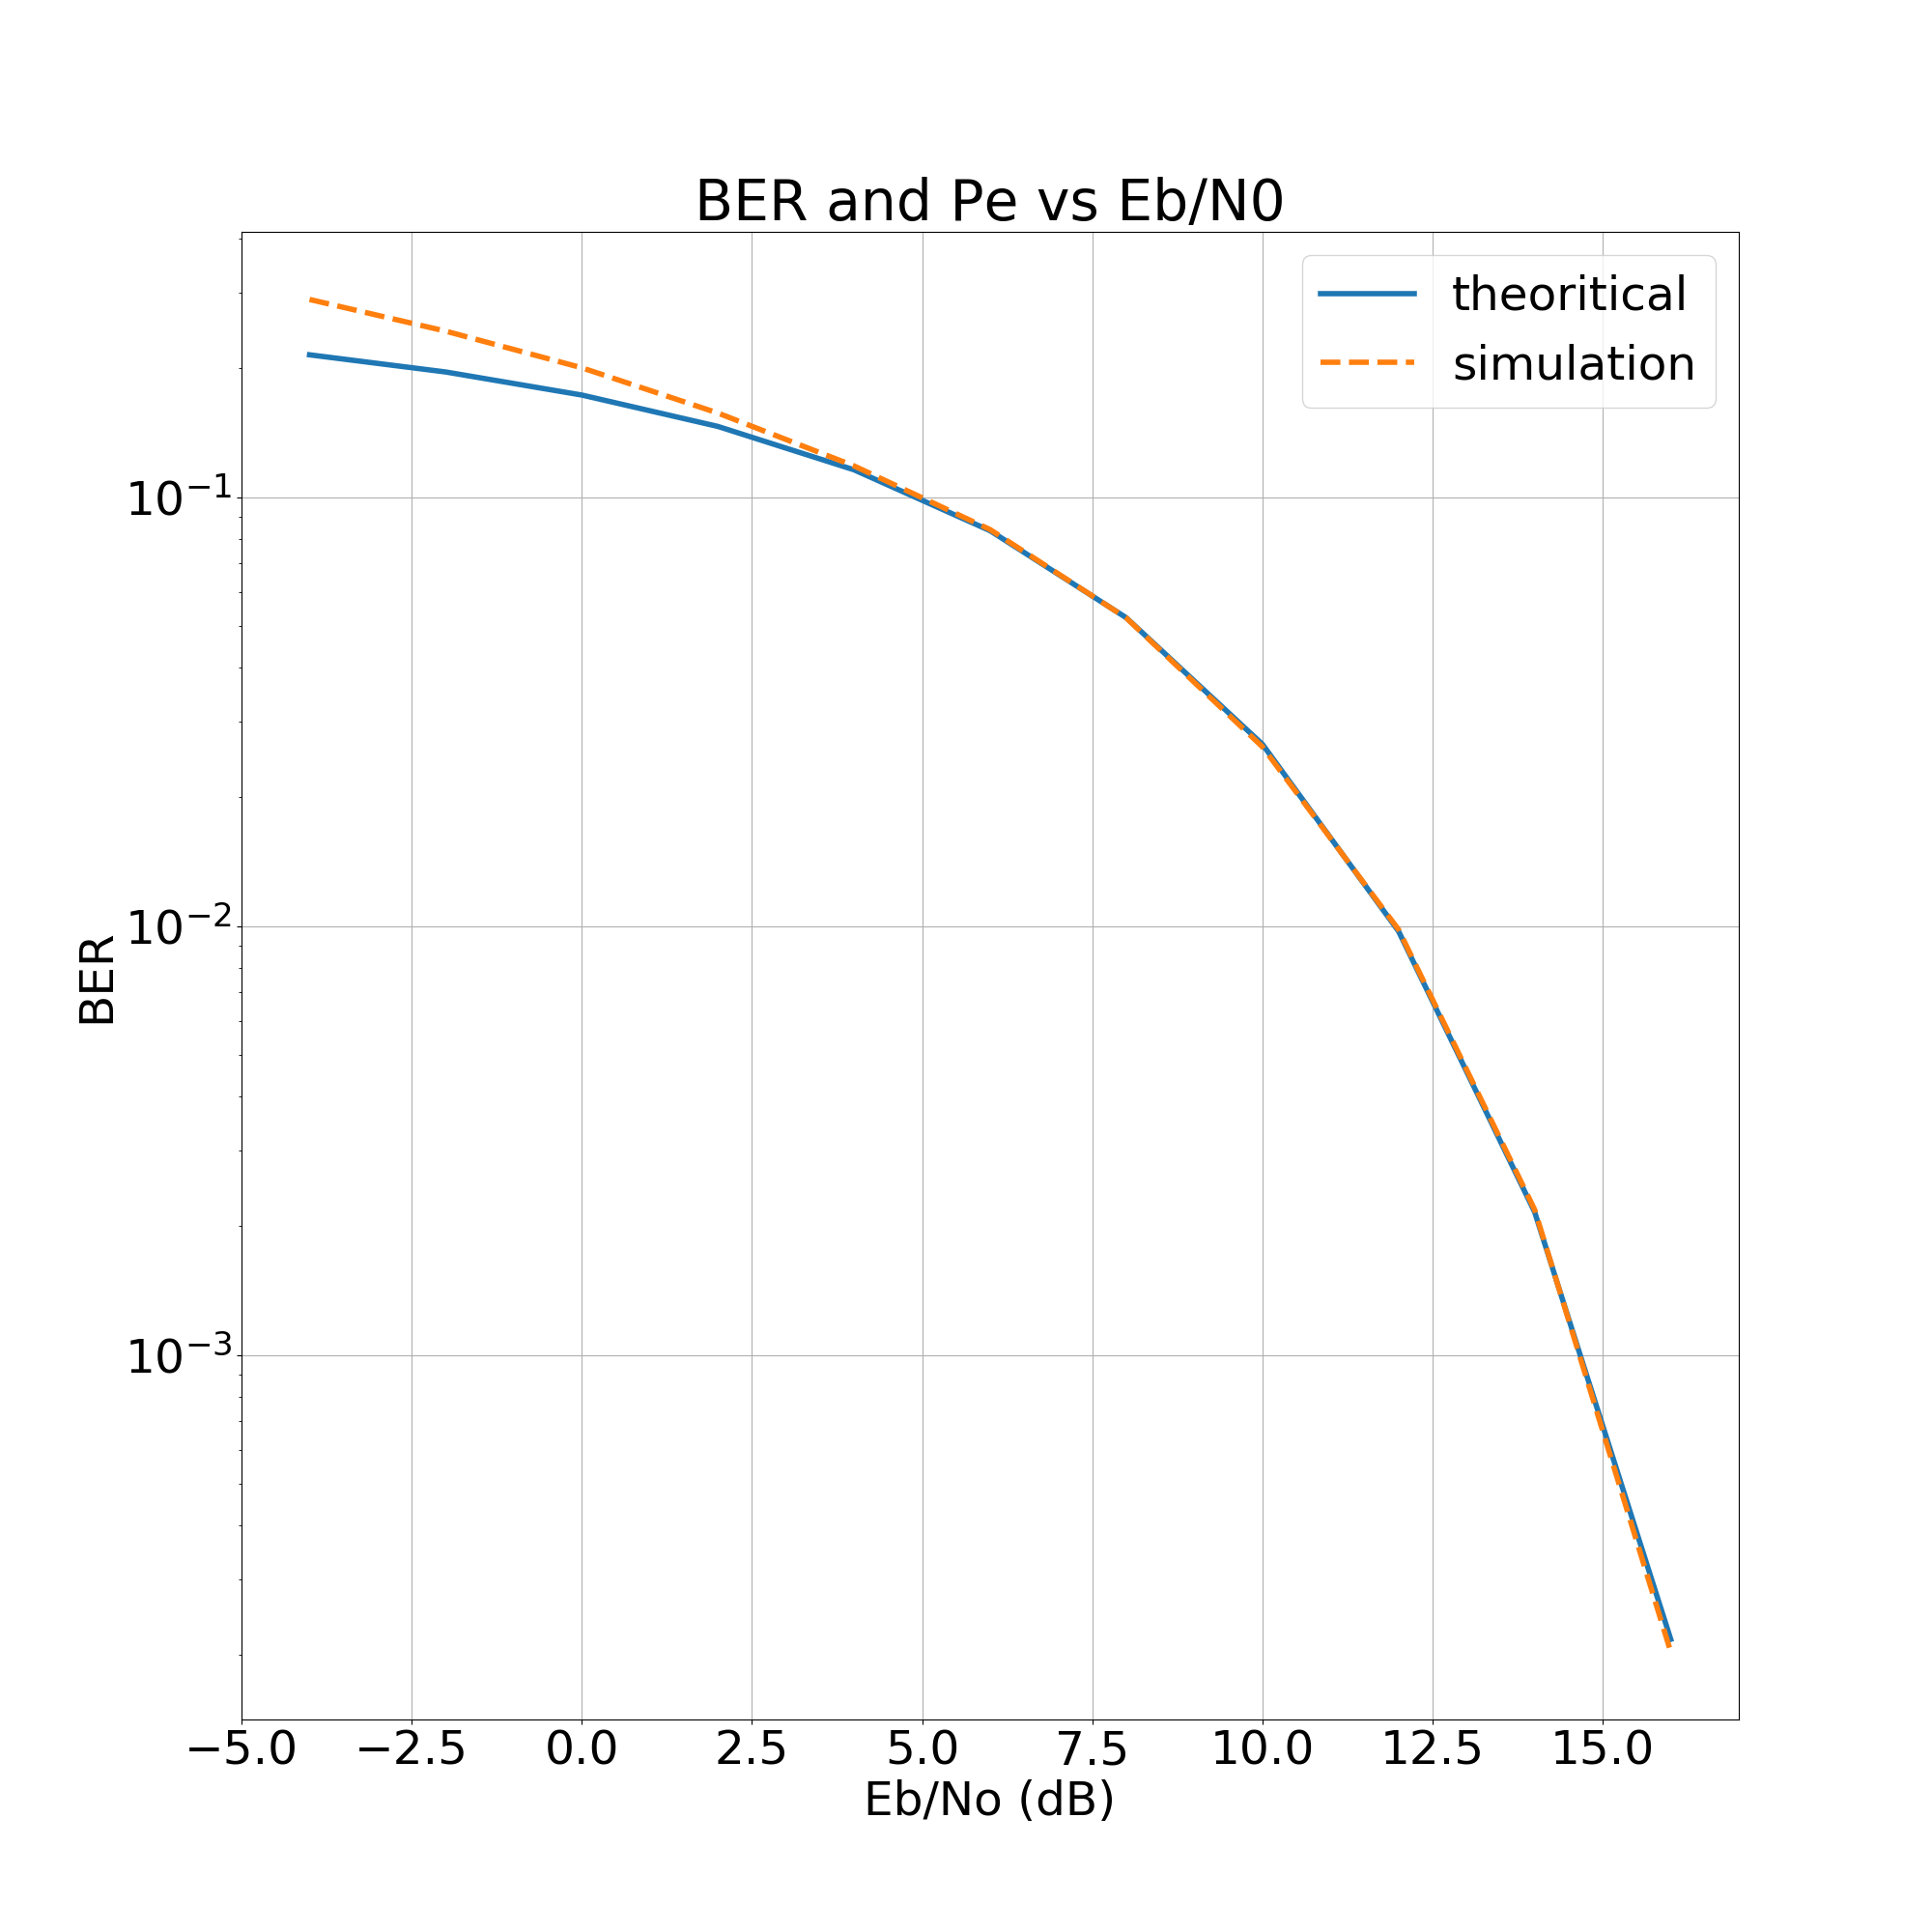
\includegraphics[width=\linewidth]{Figures/Figure_1.png}
            \caption{BER vs Eb/N0}
            \label{fig:BER}
        \end{figure}

    \subsection{Probelm 5}
        The answer is NO,
        We can't transmit at Rate 1 Mbps with bandwidth 0.5 MHz in passband transmition.

        The minimum M required: 16
        Only bit by bit transmittion is allowed.

        GIVEN:
        \begin{equation*}
            Bt = 2Rs
        \end{equation*}
        \begin{equation*}
            Rb = 1 Mbps
        \end{equation*}
        \begin{equation*}
            BW = 0.5 MHz
        \end{equation*}
        \begin{equation*}
            M = 3
        \end{equation*}

        REQUIRED:
        \begin{equation*}
            BW =? 2 * Rs
        \end{equation*}
        \begin{equation*}
            BW =? 2 * \frac{Rb}{\log_2 M}
        \end{equation*}
        \begin{equation*}
            BW =? 1Mbps * \frac{2}{3}
        \end{equation*}

        The Answer is: NO it can not be transmitted
        
        \begin{equation*}
            0.5MHz =? 1Mbps * \frac{2}{\log_2 M}
        \end{equation*}
        \begin{equation*}
            4MHz =? \log_2 M
        \end{equation*}

        and Minimum M alowed is:
        \begin{equation*}
            M = 16
        \end{equation*}
        
    \subsection{Probelm 6}
        Both of them satisfy the Gray Encoding criterion.

        Because at the two examples only one bit is changed in each transition from symbol to the next one.

    \newpage

    \section{Part 2: Information Theory}
        Cyclic Codes.
    \subsection{Definition of Cyclic Codes}
    Cyclic Codes are block codes that follow the property of linearity because they are subset of Linear codes,
    and also they have to follow the property of shifting where the circular i shift to the left (or n-1 shift to the right) always
    result in another word that belongs to the code words.
    
    They are studied usually in polynomial form because it's easier to represent them as coefficients of
        polynomials.
    {\renewcommand\labelitemi{}
    \begin{itemize}
        \item They are defined as $C(x) = (n, k)$ it means the message has $k$ bits
                and the code vector is $n$ bits.
        \item $C(x)$ are defined with the help of generator polynomial $g(x)$.
        \item The degree of $g(x)$ is equal to the number of parity-check digits of the code.
        \item There are total of $2^k$ code polynomials in $C(x)$.
        \item They are error-correction codes, used earlier to transmit images of planets.
        \item They have algebric properties that help detecting and correcting errors.
        \item Cyclic codes can be used to correct errors, it can be generalized to correct
        burst of errors, not just one bit.
        \item For example the set of [000, 1111, 0110, 1001]:
                
                They follow the Linearity property, but not the Cyclic Shift property,
                therefore they can't be considered a valide Cyclic Codes.
        \item Another Example the set of [0000, 1111, 0101, 1010]:
                
                They follow both the linearity and cyclic shift property.
                Because, when adding any two of them it will result in another (third) codeword
                that lies in the finite list.
    \end{itemize}
    

    \subsection{Systematic CodeWords:}
        In Systematic Codewords $C(x) = \left[ message, parity\right]$ this means, each
        generated codeword's first $k$ bits are the message that got us that codeword
        while the remaining $n-k$ bits are the parity check of the codeword.

        Systematic Codewords follow the following conditions:
        \begin{equation*}
            C(x) = x^{n-k} m(x) + p(x)
        \end{equation*}
        Where:
        \begin{equation*}
            p(x) = Rem \left[ \frac{x^{n-k} m(x)}{g(x)} \right]
        \end{equation*}

        and,

        $C(x)$ is codeword polynomial
        
        $m(x)$ is message polynomial
        
        $g(x)$ is generator polynomial

        \vspace{0.5cm}
        Example: Constructing a Systematic Cyclic Codes (7,4), using generator polynomial
        $g(x) = x^3 + x^2 +1$ , with message $[1 0 1 0]$.
        \vspace{0.5cm}
        
        Answer:

        $m(x) = x^3 + x$
        
        $p(x) = Rem \left[ \frac{ x^{3} *\left(x^3 + x\right) }{\left( x^3 + x^2 +1\right)} \right]$

        From division:

        $p(x) = 1$

        therefore,

        $C(x) = x^3 * \left(x^3 + x\right) + 1$
        
        $C(x) = x^6 + x^4 + 1$
        
        $C(x) = \left[1010001\right]$
        
    {\renewcommand\labelitemi{}
    \begin{itemize}
        \item You may notice that the message $m(x) = 1 0 1 0$ and the first $k$ bits in the generated
            codeword is also $1010$
        \item Will the rest of the codeword is the parity check.
    \end{itemize}

        
    \subsection{Relation between generator polynomial and generator matrix:}
        At the last section we've introduced the difinition of generator polynomial
        such that $g(x) =x^3 + x^2 +1 $, this polynomial is unique and we can derive all the other
        codewords from it by multiplying with the various messages allowed.

    {\renewcommand\labelitemi{}
    \begin{itemize}
        \item In cyclic code $C$, the generator matrix's dimentsions is $[n,k]$
            $n$ number of columns and $k$ number of rows.
        \item Generator Matric $[G]$ is composed of $[I,P]$, $I$ is the identity matrix
            with dimentsions of $[k,k]$
            while $P$ is the parity matrix with the dimentsions of $[k, (n-k)]$
        \item So, the main core of our problem is identifying the parity matrix, 
        and it is identified as follows:

        \begin{equation*}
            k^{th} Row = Rem \left[ \frac{x^{n-k}}{g(x)} \right]
        \end{equation*}

        \item continuing on the previous example the generator matrix will be something like this:
        \begin{equation*}
            G(x) = \left[ 
                \begin{matrix}
                1 & 0 & 0 & 0 & - & - & -\\
                0 & 1 & 0 & 0 & - & - & - \\
                0 & 0 & 1 & 0 & - & - & - \\
                0 & 0 & 0 & 1 & - & - & -                
                \end{matrix}
               \right]
        \end{equation*}

        so, to calculate the parity matrix we'll solve the following equations:

        \begin{equation*}
            1^{st} Row = Rem \left[ \frac{x^{6}}{ x^3 + x^2 +1} \right]
        \end{equation*}
        \begin{equation*}
            1^{st} Row = x^2 +1 = [1 0 1]
        \end{equation*}

        \begin{equation*}
            2^{nd} Row = Rem \left[ \frac{x^{5}}{ x^3 + x^2 +1} \right]
        \end{equation*}
        \begin{equation*}
            2^{st} Row = x^2 +x +1 = [1 1 1]
        \end{equation*}

        \begin{equation*}
            3^{rd} Row = Rem \left[ \frac{x^{4}}{ x^3 + x^2 +1} \right]
        \end{equation*}
        \begin{equation*}
            3^{rd} Row = x^2 +1 = [1 0 1]
        \end{equation*}

        \begin{equation*}
            4^{th} Row = Rem \left[ \frac{x^{3}}{ x^3 + x^2 +1} \right]
        \end{equation*}
        \begin{equation*}
            4^{th} Row = x +1 = [0 1 1]
        \end{equation*}

        therefore the final matrix will be:

        \begin{equation*}
            G(x) = \left[ 
                \begin{matrix}
                1 & 0 & 0 & 0 & 1 & 0 & 1\\
                0 & 1 & 0 & 0 & 1 & 1 & 1 \\
                0 & 0 & 1 & 0 & 1 & 0 & 1 \\
                0 & 0 & 0 & 1 & 0 & 1 & 1                
                \end{matrix}
               \right]
        \end{equation*}


    \end{itemize}

    \subsection{Cyclic Codes Encoding Procedure}
    As we already know the code word consists of [message, parity], \textit{message} is what the system gives
        as an input, \textit{parity} is what gets we encode, each code word is $N$ bits,
        the first $K$ of them are the message, while the rest $N-K$ are the parity.
    
    Initially the values of the flip-flops is set to the generator polynomial, and with every bit
        inserted from the message input the new value of the flip-flop is decided then, whether it will 
        be the same or the result from the outcome of the XOR (Add) operation.

    Shown in fig. \ref{fig:encoder}, a simple encoder of $k$ bits parity for codewords.
    \begin{figure}[h!]
        %I put \linewidth into the brackets, which means the picture will be scaled to fit the width of the document.
        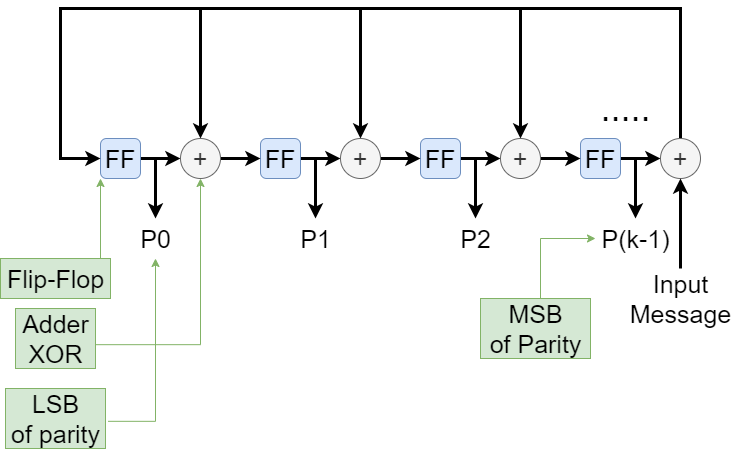
\includegraphics[width=\linewidth]{Figures/cyclic_codes_encoding.png}
        \caption{Cyclic Code Encoder}
        \label{fig:encoder}
    \end{figure}

    The Initial value of these branches is dominated by the generator polynomial, so if Initially one
        of these branches is equal to zero, it will remain zero for the rest of the operation,
        and pass the value of the previous flip-flop to the next one without making any additions.

    The input value of each flip-flop could be the previous value of another flip-flop, the outcome
        of the addition process or -in case of the first flip-flop- the coutcome of the input message bit
        XORed with the MSB parity bit.
    
    This process goes on and on for all of the input message bits, until the last one of them,
        and then the remaining values of parity is the actual encoding bits we are looking for,
        and our codeword is the [message, parity].
    \newline

    Below is an example, illustrating more on that:
        \begin{itemize}
            \item If polynomial generator is $g(x) = 1 + x + x^3$
            \item message is [1110]
            \item we are asked to generate codeword for it..
        \end{itemize}

    Solution:
        \begin{itemize}
            \item the generator is $1101$ and that's the init. value of the branches.
        \end{itemize}
    
        \begin{center}
            \begin{tabular}{||c c c c||} 
            \hline
            msg & P0 & P1 & P2 \\ [0.5ex] 
            \hline\hline
            - & 0 & 0 & 0 \\ 
            \hline
            1 & 1 & 1 & 0 \\
            \hline
            1 & 1 & 0 & 1 \\
            \hline
            1 & 0 & 1 & 0 \\
            \hline
            0 & 0 & 0 & 1 \\ [1ex] 
            \hline
           \end{tabular}
           \end{center}
        \begin{itemize}
            \item as one can see:
            \item at the first row, the init value of the polynomials is zeros
            \item at the second row, after inputing 1 from the message,
                $P0$ value is $XOR$ of the input message bit and $P2$,
                $P1$ value is $XOR$ of old $P0$ and $1$ from the branch,
                $P2$ value is the same as old $P1$ because its branch is zero.
            \item and so on until we reach the end of the input message's bits.
        \end{itemize}
    
    input message is [1110] and parity bits is [001]
    
    So the final codeword is [1110001]
    %%%%%%%%%%%%%%%%%%%%%%%%%%APPENDIX%%%%%%%%%%%%%%%%%%%%%%%%%%
    \newpage

    \section{Appendix: Main Code for part 1}

    \lstset{language=Python}
    \lstset{frame=lines}
    % \lstset{caption={Main Code for part 1}}
    % \lstset{label={lst:code_direct}}
    \lstset{basicstyle=\footnotesize}
    \lstinputlisting[language=Python]{../main.py}

    
\end{document}

